\documentclass[10pt,a4paper]{book}
\usepackage[utf8]{inputenc}
\usepackage{amsmath}
\usepackage{amsfonts}
\usepackage{amssymb}
\usepackage{graphicx}
\usepackage{listings}
\usepackage{xcolor}
\usepackage[left=3.00cm, right=3.00cm, top=2.00cm, bottom=2.00cm]{geometry}
\definecolor{codegreen}{rgb}{0,0.6,0}
\definecolor{codegray}{rgb}{0.5,0.5,0.5}
\definecolor{codepurple}{rgb}{0.58,0,0.82}
\definecolor{backcolour}{rgb}{0.95,0.95,0.92}

\lstdefinestyle{mystyle}{
	backgroundcolor=\color{backcolour},   
	commentstyle=\color{codegreen},
	keywordstyle=\color{magenta},
	numberstyle=\tiny\color{codegray},
	stringstyle=\color{codepurple},
	basicstyle=\ttfamily\footnotesize,
	breakatwhitespace=false,         
	breaklines=true,                 
	captionpos=b,                    
	keepspaces=true,                 
	numbers=left,                    
	numbersep=5pt,                  
	showspaces=false,                
	showstringspaces=false,
	showtabs=false,                  
	tabsize=2
}

\lstset{style=mystyle}
\begin{document}
	\begin{center}
		\Large {\textbf{Relazione esperienza flessione}}
    \end{center}
\textbf{Gruppo 30: }Bigi Giulia, Cipriani Stella, Foglia Alex, Mallamaci Benedetto.
\mbox{}\\*
\section*{Descrizione dell'esperienza}
Quello di corpo rigido è un vincolo ideale, in realtà ogni solido cede all'azione delle forze e dei momenti che tendono a deformarlo. Le forze possono essere di:
\begin{itemize}
	\item Trazione o compressione;
	\item Taglio;
\end{itemize}
Mentre i momenti possono essere di:
\begin{itemize}
	\item Torsione;
	\item Flessione.
\end{itemize}
Lo scopo dell'esperienza è quello di misurare il \textbf{modulo di Young} di un materiale mediante la misura diretta della flessione di un parallelepipedo.\\*
La sollecitazione di flessione si osserva su un corpo elastico avente un estremo fissato, che chiamiamo \emph{base fissa}, quando un sistema di forze agenti su di esso è tale per cui la loro risultante è nulla, mentre il momento delle forze rispetto al piano della base fissa è perpendicolare ad essa e non nullo.\\*\\*
L'apparato sperimentale è composto da due coltelli paralleli posti a una distanza $L$ i quali poggiano su di una guida orizzontale. La sbarretta composta dal materiale di cui vogliamo misurare il modulo di Young è poggiata sopra i due coltelli, e nel punto centrale della medesima vi è appeso un supporto sopra al quale si posizioneranno i pesi. In particolare, siamo interessati a misurare la \emph{freccia di flessione}, ossia quel tratto $f$ del quale si è spostato il punto centrale della sbarretta quando vi applichiamo un peso noto.
\begin{figure}[h]
	\centering
	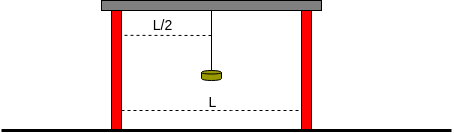
\includegraphics[width=0.7\linewidth]{appexp}
	\caption{Apparato sperimentale}
	\label{fig:appexp}
\end{figure}
\begin{figure}[h]
	\centering
	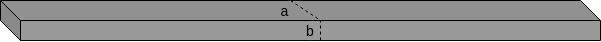
\includegraphics[width=0.7\linewidth]{sbarretta}
	\caption{Sbarretta}
	\label{fig:sbarr}
\end{figure}
\\*\\*
Siamo interessati a misurare $f$ in quanto sappiamo che, per una data coppia freccia-peso $(f_i, P_i)$, vale:
$$
f_i = c\;P_i
$$
Dove $c$ è detta \emph{costante di flessione}.\\*
Il modulo di Young è dato dalla relazione:
$$
E = \frac{L^3}{4ab^3c}
$$
Per determinare $c$ effettueremo due misure di quote $h_0, h_i$, come specificato più avanti, e la misura del peso $P_i$ associato a ciascuna coppia di quote. Per poter infine determinare $E$ dobbiamo misurare anche le lunghezze $L, a, b$.\\*
Nell'eseguire l'esperimento dobbiamo assicurarci che i coltelli siano perfettamente paralleli e la sbarretta orizzontale, che assumiamo inoltre omogenea nella sua composizione materiale.\\*
Nell'eseguire le misure di quota, dovremo ottenere un valore $h_0$ corrispondente alla quota del tratto centrale della sbarretta a supporto scarico, e un valore $h_i$ corrispondente alla stessa quota quando invece è applicato un peso sul supporto. Otterremo quindi:
$$
f_i = c\;P_i
$$
$$
h_0 - h_i = c\;Pi
$$
$$
h_i = h_0 - c\;Pi
$$
Osserviamo che questa espressione è valida finchè le deformazioni subite dalla sbarretta rimangono nella regione di proporzionalità.
\section*{Elenco degli strumenti}
Per poter effettuare le misure di quota $h_i$ e $h_0$, sfruttiamo un truschino costituito da un'asta graduata disposta in verticale
accoppiata a un laser che scorre su di essa. Il laser permette di misurare quote a distanza. L'errore di sensibilità della scala graduata è di 0.02 mm.\\*
I pesi $P_i$ vengono misurati sfruttando una bilancia elettronica usata come dinamometro. La bilancia ha un errore di linearità di 0.03 g e un errore di riproducibilità di 0.01 g.\\*
La lunghezza $a$ della sbarretta viene misurata mediante un calibro ventesimale, quindi con errore di sensibilità pari a 0.05 mm. La lunghezza $b$ viene misurata con un palmer avente errore di sensibilità 0.01 mm e un offset medio di -0.01 mm.\\*
$L$ viene infine misurata con una riga graduata dotata di due scale, una con errore di sensibilità 0.5 mm, e un'altra 1 mm.
\begin{center}
\begin{tabular}{|c|c|c|c|}
	\hline 
	\textbf{Strumento} & \textbf{Grandezza} & \textbf{Errore a priori} & \textbf{Offset} \\ 
	\hline 
	Truschino & Quote $h_i$ & 0.02 mm & -  \\ 
	\hline 
	Calibro & Lunghezza $a$ & 0.05 mm & - \\ 
	\hline 
	Palmer & Lunghezza $b$ & 0.01 mm & -0.01 mm \\ 
	\hline 
	Riga graduata & Lunghezza $L$ & 1 mm & - \\ 
	\hline 
	Bilancia & Pesi $P_i$ & 0.04 g & - \\ 
	\hline 
\end{tabular}
\end{center}
Per quanto riguarda la riga graduata, abbiamo scelto di usare la scala con errore di sensibilità 1 mm a causa delle procedure di misura che non permettono di apprezzare il mezzo millimetro.
\section*{Descrizione delle procedure}
Le misure dirette che occorre effettuare riguardano le dimensioni della sbarretta, i pesi, e le quote del tratto centrale della sbarretta.\\*
Utilizziamo una livella per verificare la posizione orizzontale della sbarretta quando posta sopra i coltelli, e quindi la loro perpendicolarità rispetto alla guida su cui poggiano. Poniamo in corrispondenza del tratto centrale un cavaliere sul quale è inciso un traguardo orizzontale. Questa linea servirà come riferimento per le misure di quota.
\begin{figure}[h]
	\centering
	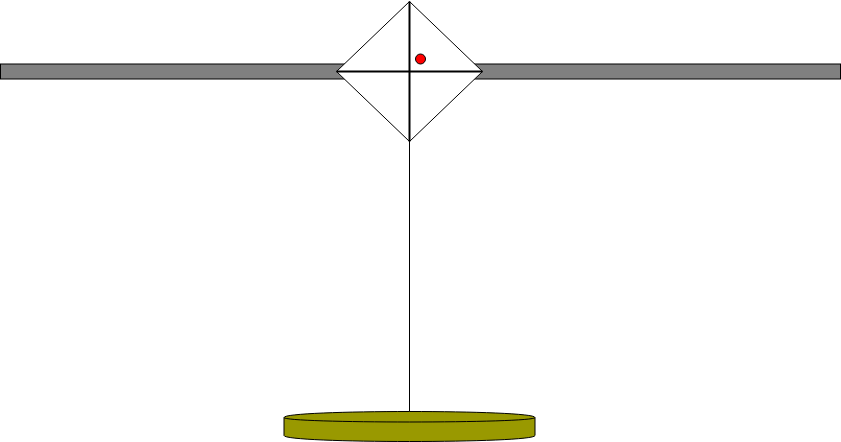
\includegraphics[width=0.7\linewidth]{cavaliere}
	\caption{Traguardo su cavaliere e laser del truschino}
	\label{fig:cavaliere}
\end{figure}
Per poter essere ragionevolmente sicuri di misurare effettivamente le variazioni di quota che ci interessano, dobbiamo prestare assoluta attenzione al fatto che il laser sia sempre perpendicolare rispetto all'asta graduata del truschino, e che la base di quest'ultimo rimanga sempre perfettamente orizzontale. Usiamo una livella per verificare questa condizione.\\*
Una volta realizzato l'apparato sperimentale utilizziamo un pennarello per marcare la posizione dei coltelli sulla sbarretta e misuriamo mediante la riga graduata la lunghezza $L$. Sempre sulla sbarretta misuriamo le dimensioni $a,b$ usando rispettivamente il calibro e il palmer, avendo accortezza di effettuare misure ripetute in punti diversi, di modo da tener conto della non perfetta forma omogenea della sbarretta.\\*
Posizioniamo quindi la sbarretta sui coltelli e iniziamo a misurare le quote della sbarretta sfruttando gli spostamenti micrometrici sul truschino, e i pesi che applichiamo.\\*
È importante verificare di non essere usciti dalla regione di proporzionalità, altrimenti staremo alterando il significato fisico dell'esperienza. A tale scopo misuriamo la quota $h_0$ a supporto scarico, e la quota $h_0'$ nuovamente a supporto scarico dopo aver effettuato la misura $h_i$. Se siamo rimasti nella regione elastica, allora $h_0'$ dovrà trovarsi nell'intervallo $h_0 \pm \Delta h_0$, dove $\Delta h_0$ è l'incertezza su $h_0$, che otterremo come scarto massimo tra misure ripetute.\\*
La regione di proporzionalità è ridotta rispetto alla regione elastica, quindi terremo in considerazione solamente valori di $h_i$ tali per cui vale:
$$
h_i = h_0 - c\;P_i
$$
\section*{Stima a priori delle incertezze}
Per quanto riguarda la stima dell'errore a priori sulle misure dirette, ci è sembrato ragionevole supporre di essere stati attenti a eliminare le cause di errore sistematico.\\*
Si suppone di avere una sbarretta di lunghezza $L = (300 \pm 1)$ mm, avente $a = (20.00 \pm 0.05)$ mm e $b = (2.00 \pm 0.01)$ mm. I valori:\\*
$$
\Delta L = 1\;mm
$$
$$
\Delta a = 0.05\;mm
$$
$$
\Delta b = 0.01\;mm
$$
Li abbiamo dedotti considerando l'errore di sensibilità degli strumenti che utilizzeremo durante lo svolgimento dell'esperienza, mentre i valori di
$$
L = 300\;mm
$$
$$
a = 20\;mm
$$
$$
b = 2\;mm
$$
Li abbiamo immaginati come plausibili per la sbarretta che utilizzeremo.\\*
Per la bilancia assumiamo un'incertezza a priori sul peso pari a $\Delta P = 0.04\;g = 0.00004\;kg = 4\;10^{-5}\;kg$, che corrisponde all'incertezza dello strumento scelto.\\*
Applicando il metodo della derivata logaritmica all'espressione $ E = \frac{L^3}{4ab^3c} $ possiamo determinare l'incertezza relativa $\frac{\Delta E}{E}$. 
Osserviamo che per poter determinare questa quantità è necessario conoscere anche la quantità $\frac{\Delta c}{c}$, che possiamo stimare attraverso la relazione:
$$
\left|\frac{\Delta c}{c}\right| = 2 \left|\frac{\Delta h}{h_0 - h_{max}}\right| + \left|\frac{\Delta P_{max}}{P_{max}}\right|
$$
Dove $P_{max}$ è il peso massimo applicabile alla sbarretta senza uscire dalla regione di proporzionalità, e $h_{max}$ la quota associata al peso $P_{max}$.\\*\\*
Supponiamo che la sbarra sia di alluminio:
$$
P_{max} = \sigma_p \frac{ab^2}{L} = 15 \frac{kg_p}{mm^2} \frac{20mm\;(2mm)^2}{300mm} = 4.0 kg_p
$$
$$
c = \frac{L^3}{4E_{Al}ab^3} = \frac{(300\;mm)^3}{28\;10^3\frac{kg_p}{mm^2}\;20\;mm\;(2\;mm)^3} \approx 6.03\;\frac{mm}{kg_p}
$$
Le misure di quota verranno effettuate mediante un truschino avente errore a priori $\Delta h = 0.02\;mm$. Utilizziamo questo valore per la stima a priori delle incertezze.\\*
Supponiamo infine $h_0 = 0 mm$ e:
$$
h_{max} = h_0 - c\;P_{max} = -6.03\frac{mm}{kg_p}\;4\;kg_p = -24.12\;mm
$$
Otteniamo:
$$
\left|\frac{\Delta c}{c}\right| = 2 \left|\frac{0.02\;mm}{6.03\;mm}\right| + \left|\frac{4\;10^{-5}\;kg_p}{4\;kg_p}\right| \approx 0.003 + 10^{-5} \approx 0.003
$$
A questo punto possiamo ricavare la stima dell'incertezza a priori:
$$
\frac{dE}{E} = d\;ln(E) = d\;ln\left(\frac{L^3}{4ab^3c}\right) =
$$
$$
= d\;(ln(L^3) - ln(4ab^3c)) =
$$
$$
= d(3\;ln(L) - ln(4) - ln(a) - 3\;ln(b) - ln(c)) =
$$
$$
\frac{3}{L}\;dL - \frac{1}{a}\;da - \frac{3}{b}\;db - \frac{1}{c}\;dc
$$
Passando ai valori finiti:
$$
\frac{\Delta E}{E} = 3\frac{\Delta L}{L} + \frac{\Delta a}{a} + 3 \frac{\Delta b}{b} + \frac{\Delta c}{c}
$$
$$
\frac{\Delta E}{E} = 3\frac{1mm}{300mm} + \frac{0.05mm}{20mm} + 3 \frac{0.01mm}{2mm} + 0.003
$$
$$
\frac{\Delta E}{E} = 0.01 + 0.0025 + 0.0015 + 0.003 = 0.017 \approx 0.02
$$
Stimiamo a priori un errore relativo di circa il $2$\% con il contributo preponderante di $\frac{\Delta L}{L}$.\\*
Questo ci suggerisce che la misura di $L$ sia la parte più critica dell'esperienza, cosa che appare ragionevole considerando la procedura di misura e lo strumento utilizzato.
\section*{Dati sperimentali}
\small
\begin{tabular}{|c|c|c|c|c|c|c|c|c|}
	\hline 
	\textbf{Grandezza} & $L$(mm) & $a$(mm) & $b$(mm) & offset(mm) & $h_0$(mm) & $P_i$(g\textsubscript{p})& $h_i$(mm) & $h_0'$(mm) \\ 
	\hline 
	\textbf{Strumento} & Riga graduata & Calibro & Palmer & Palmer & Truschino & Bilancia & Truschino & Truschino \\ 
	\hline 
	\textbf{Valori}
	& 300.0  & 23.30 & 1.99 & 0.00 & 230.60 & 46.52  & 230.24 & 230.52 \\ 
	\hline 
	& 299.0  & 23.20 & 1.99 & -0.02 & 230.58 & 114.67 & 229.96 & 230.50 \\ 
	\hline 
	& 299.0  & 23.30 & 1.97 & 0.00 & 230.46 & 230.75 & 229.34 & 230.56 \\ 
	\hline 
	&  & 23.15 & 2.00 & -0.02 & 230.54 & 366.94 & 228.54 & 230.54 \\ 
	\hline 
	&  & 23.30 & 2.03 & -0.02 & 230.56 & 462.75 & 228.02 & 230.54 \\ 
	\hline 
	&  & 23.25 & 1.99 &  & 230.50 & 509.16 & 227.88 & 230.60 \\ 
	\hline 
	&  & 23.30 & 2.03 &  &  & 646.86 & 227.04 & 230.46 \\ 
	\hline 
	&  & 23.30 & 2.00 &  &  & 713.49 & 226.78 & 230.58 \\ 
	\hline 
	&  &  &  &  &  & 829.50 & 226.16 & 230.48 \\ 
	\hline 
	&  &  &  &  &  & 925.29 & 225.56 & 230.52 \\ 
	\hline 
\end{tabular}
\normalsize
\section*{Elaborazione dei dati}
Determiniamo la miglior stima di $L$ come la media tra le misure di $L$:
$$
\overline{L} = \frac{300.0\;mm+299.0\;mm+299.0\;mm}{3} = 299.3\;mm
$$
E l'incertezza $\Delta L$ rimane l'incertezza dello strumento, poichè lo scarto massimo:
$$
\Delta L = |{L_{max}-\overline{L}}| = |{300\;mm - 299.3\;mm}| = 0.7\;mm < 1\;mm \Rightarrow \Delta L = 1\;mm
$$
Quindi
$$
L = (299.3 \pm 1.0)\;mm
$$
Ripetiamo questa procedura anche per determinare le migliori stime e le incertezze su offset, $a$, $b$, e $h_0$:\\*\\*
Offset = $\frac{-0.02\;mm - 0.02\;mm - 0.02\;mm}{5} = -0.01\;mm$
$$
\overline{a} = 23\;mm + \frac{0.30\;mm + 0.20\;mm + 0.30\;mm + 0.15\;mm + 0.30\;mm + 0.25\;mm + 0.30\;mm + 0.30\;mm}{8} = $$
$$23\;mm + 0.25\;mm = 23.25\;mm
$$
$$
\Delta a = |a_{max} - \overline{a}| = |23.15\;mm - 23.25\;mm| = 0.10\;mm
$$
$$
a = (23.25 \pm 0.10)\;mm
$$
$$
\overline{b} = \frac{1.99\;mm + 1.99\;mm + 1.97\;mm + 2.00\;mm + 2.03\;mm+1.99\;mm+2.03\;mm+2.00\;mm}{8} = 2.00\;mm
$$
Considerando il contributo dell'offset:
$$
\overline{b} = 2.00\;m - (-0.01\;mm) = 2.01\;mm
$$
$$
\Delta b = |b_{max} - \overline{b}| = |1.97\;mm - 2.01\;mm| = 0.04\;mm
$$
$$
b = (2.01 \pm 0.04)\;mm
$$
$$
\overline{h_0} = 230\;mm + \frac{0.60\;mm + 0.58\;mm+0.46\;mm+0.54\;mm+0.56\;mm+0.50\;mm}{6} =
$$
$$ 230\;mm + 0.54\;mm = 230.54\;mm
$$
$$
\Delta h_0 = |h_{0_{max}} - \overline{h_0}| = |230.46\;mm - 230.54\;mm| = 0.08\;mm
$$
$$
h_0 = (230.54 \pm 0.08)\;mm
$$
Per assicurarci che durante le misure non abbiamo mai superato la regione elastica verifichiamo che tutte le misure $h_0'$ stiano nell'intervallo chiuso:
$$
[230.54 - 0.08,230.54 + 0.08] = [230.46, 230.62]
$$
Fatto che si verifica.\\*
Applichiamo il metodo dei minimi quadrati a ciascuna coppia $(P_i, h_i)$ misurata, ottenendo:
$$
h_0 = (230.53 \pm 0.03)\;mm
$$
$$
c = (0.00532 \pm 0.00006) \frac{mm}{g_p} = (5.32 \pm 0.06) \frac{mm}{kg_p}
$$
$$
\sigma^2_y = 0.002573\;mm^2 \Rightarrow \sigma_y = \sqrt{0.002573} \approx 0.05\;mm
$$
È possibile determinare $E$ attraverso la relazione funzionale:
$$
E = \frac{L^3}{4ab^3c} = \frac{(299.3\;mm)^3}{4\;23.25\;mm\;(2.01\;mm)^3\;5.32\;\frac{mm}{kg_p}} \approx 6670\;\frac{kg_p}{mm^2} = 6.67\;10^3 \;\frac{kg_p}{mm^2} 
$$
Utilizziamo l'espressione della derivata logaritmica per ricavare l'incertezza relativa a posteriori:
$$
\frac{\Delta E}{E} = 3\frac{\Delta L}{L} + \frac{\Delta a}{a} + 3 \frac{\Delta b}{b} + \frac{\Delta c}{c}
$$
In cui adesso sostituiamo le incertezze espresse come scarto massimo, e non più come errore a priori dello strumento di misura:
$$
\frac{\Delta E}{E} = 3\frac{1.0\;mm}{299.3\;mm} + \frac{0.10\;mm}{23.25\;mm} + 3 \frac{0.04\;mm}{2.01\;mm} + \frac{0.06 \frac{mm}{kg_p}}{5.32 \frac{mm}{kg_p}} \approx
$$
$$
0.010 + 0.004 + 0.060 + 0.011 = 0.085 \approx 0.09
$$
$$
\Delta E = \frac{\Delta E}{E}\;E = 0.09\;6.67\;10^3 \frac{kg_p}{mm^2} = 0.6003\;10^3 \frac{kg_p}{mm^2} \approx 0.60\;10^3
$$
Pertanto concludiamo che
$$
E = (6.67\pm0.60)10^3 \frac{kg_p}{mm^2}
$$
\section*{Conclusioni}
Confrontando il risultato di $E$ con la tabella nelle dispense, concludiamo che il materiale di cui è composta la sbarretta è alluminio, in quanto il modulo di Young $E_{Al}$ dell'alluminio:
$$
E_{Al} = 7\;10^3 \frac{kg_p}{mm^2} \in E \pm \Delta E
$$
L'errore a posteriori è aumentato rispetto alla stima a priori, infatti avevamo stimato un errore relativo a priori approssimativo:
$$
\frac{\Delta E}{E}_{priori} = 0.02
$$
E abbiamo ottenuto un errore a posteriori:
$$
\frac{\Delta E}{E}_{posteriori} = 0.09
$$
Questo risultato era comunque preventivato poichè sapevamo che con la stima a priori stavamo sottostimando l'errore delle misure dirette, assumendolo per ciascuna misura pari alla sensibilità dello strumento. La valutazione a priori aveva individuato come maggiormente critica l'operazione di misura della lunghezza $L$ mediante la riga graduata, nella stima a posteriori ci siamo accorti che in realtà il contributo preponderante all'errore veniva invece dato dalla quantità $\frac{\Delta b}{b}$, e questo ci suggerisce che probabilmente abbiamo commesso degli errori nel prendere le misure della lunghezza $b$, infatti, attraverso lo scarto massimo delle misure, abbiamo quadruplicato l'errore $\Delta b$, stimato a priori pari alla sensibilità del Palmer:
$$
\Delta b_{priori} = 0.01\;mm
$$
$$
\Delta b_{posteriori} = 0.04\;mm = 4\Delta b_{priori}
$$
Nel complesso, l'errore relativo a posteriori è aumentato del:
$$
\frac{\frac{\Delta E}{E}_{posteriori} - \frac{\Delta E}{E}_{priori}}{\frac{\Delta E}{E}_{priori}} = \frac{0.09 - 0.02}{0.02} = \frac{0.07}{0.02} = 3.5 \Rightarrow 350\%
$$
Infatti:
$$
\frac{\frac{\Delta E}{E}_{posteriori}}{\frac{\Delta E}{E}_{priori}} = \frac{0.09}{0.02} = 4.5 \Rightarrow \frac{\Delta E}{E}_{posteriori} = 4.5\frac{\Delta E}{E}_{priori}
$$
L'algoritmo dei minimi quadrati ci ha permesso di calcolare la fluttuazione media dei valori della $h_i$ rispetto alla retta dei minimi quadrati. In linea di principio dovrebbe essere, per un buon fit $\sigma_y \approx \Delta_{h_i}$. In realtà ciò non si verifica, in particolare:
$$
\Delta_{h_i} = 0.02\;mm
$$
$$
\sigma_y = 0.05\;mm
$$
Ci troviamo nella situazione in cui $\sigma_y > \Delta_{h_i}$, e questo potrebbe far pensare che non esista una relazione lineare tra i pesi e le quote della sbarretta.\\*
Una possibile interpretazione che diamo a questo fenomeno è che le misure $h_i$ sono misure singole, e pertanto poco affidabili. Di contro, misure ripetute di $h_0$ hanno dato luogo a un'incertezza intesa come scarto massimo dalla media $\Delta_{h_0} = 0.08\;mm$, valore che è pur sempre minore di $\sigma_y$ ma tale per cui la relazione lineare non verrebbe meno. Più che della effettiva non linearità della relazione fra le grandezze, siamo scettici sulla rappresentatività dell'incertezza $\Delta_{h_i}$.\\*
Questo effetto lo si nota anche nel grafico allegato, infatti la retta che abbiamo disegnato non passa per tutte le barre di incertezza degli $h_i$ misurati.\\*
Il valore di $c$ determinato graficamente vale:
$$
c_{grafico} \approx 0.005\; \frac{mm}{g_p}
$$
Questo valore è comunque in accordo a quello determinato attraverso il metodo dei minimi quadrati.
\section*{Grafico}
\begin{center}
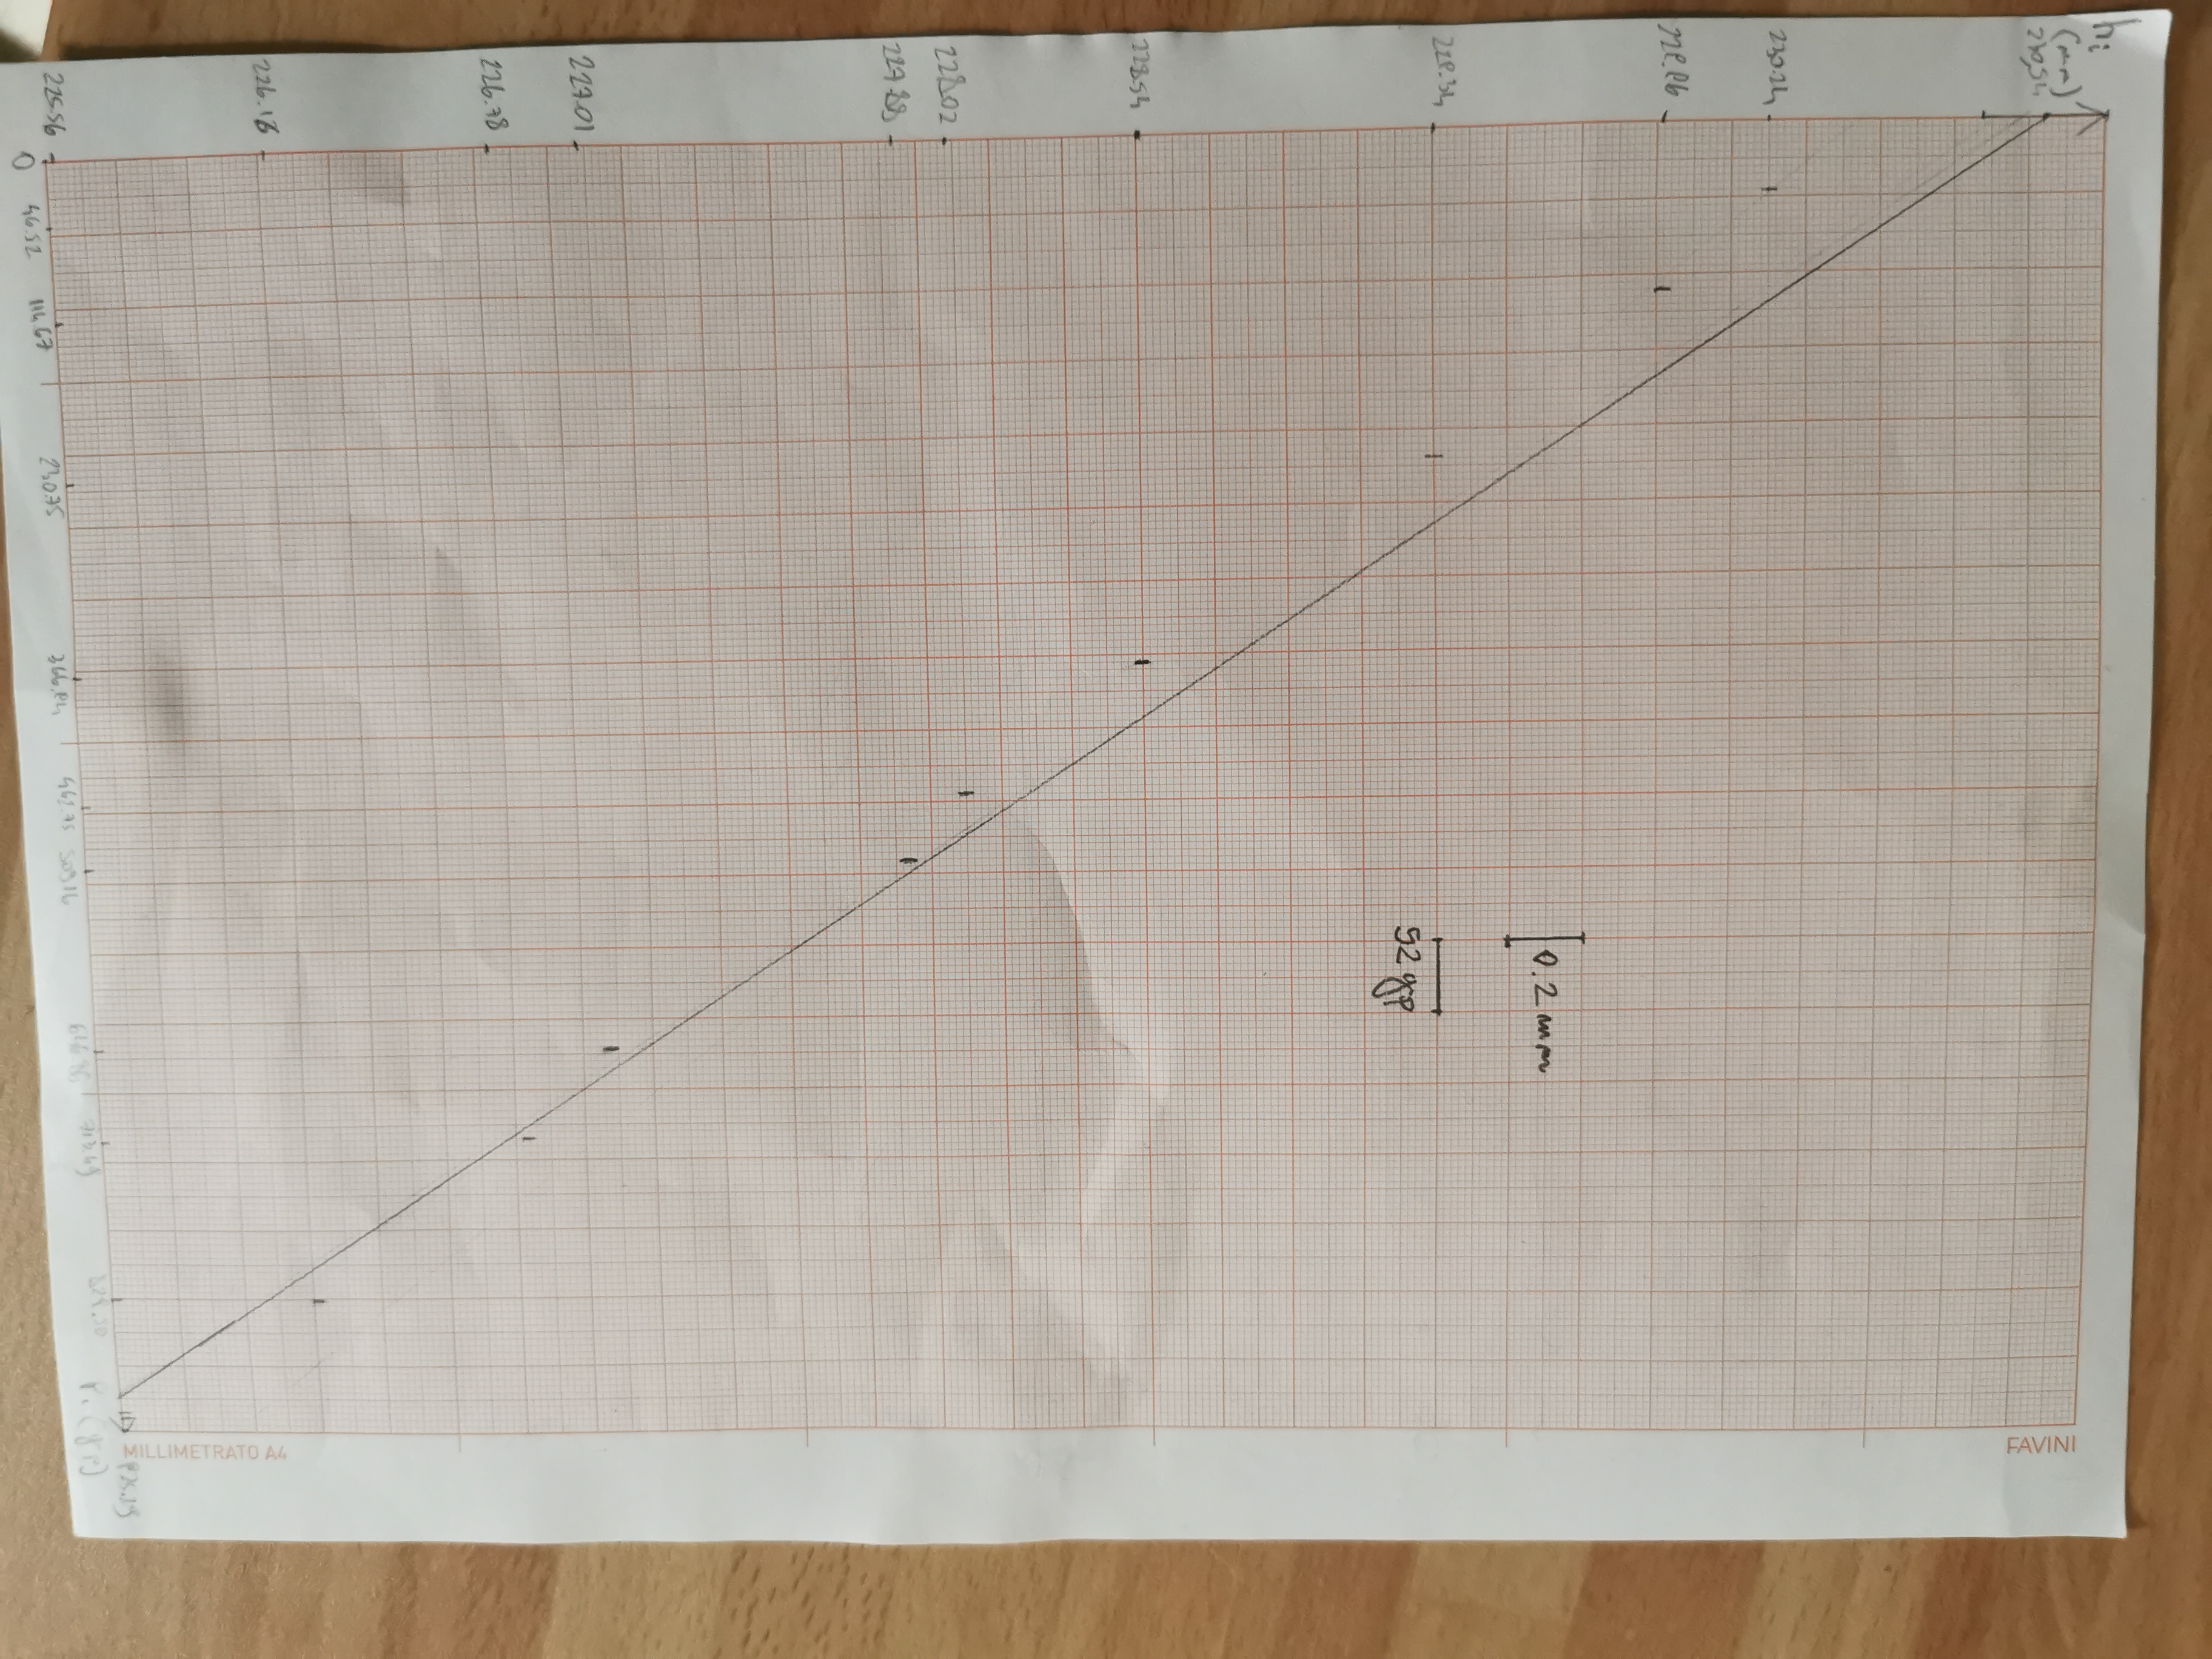
\includegraphics[scale=0.18, angle=90]{imggrafico}
\end{center}
\begin{center}
	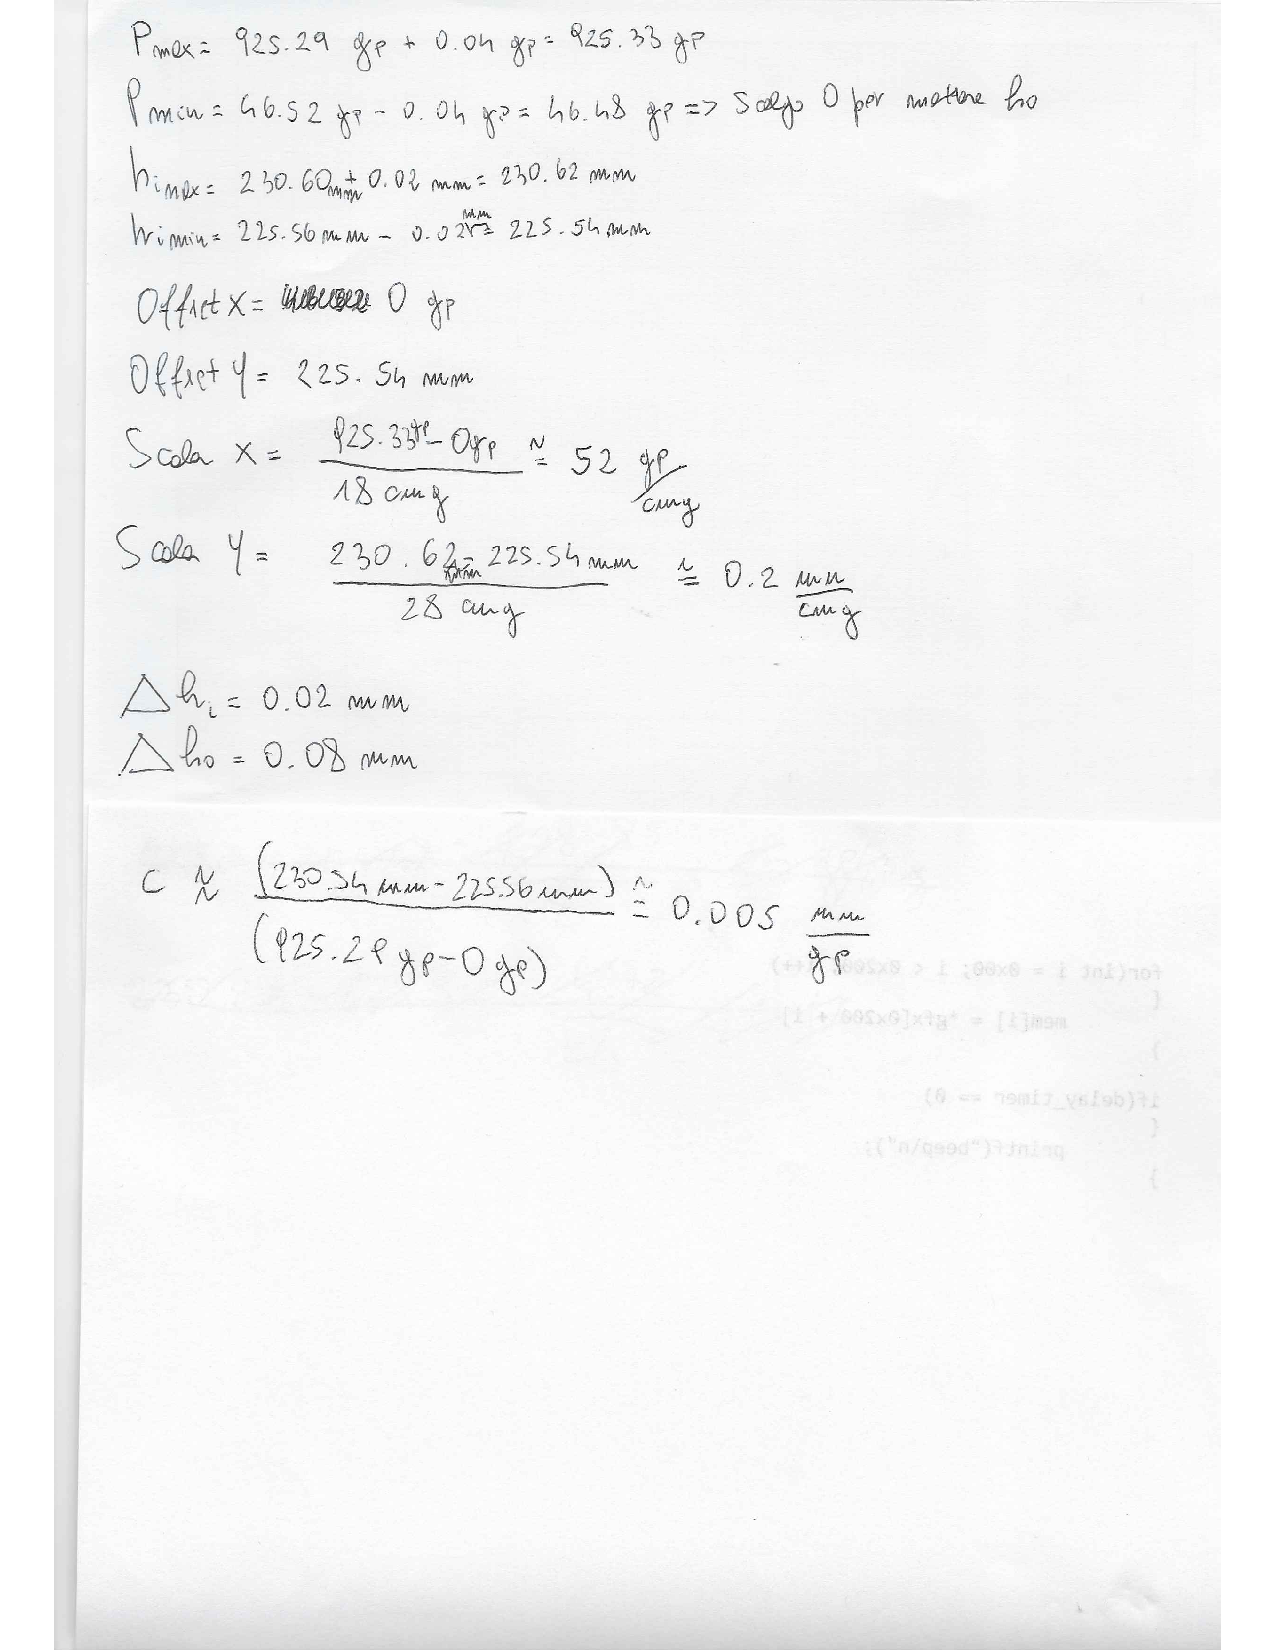
\includegraphics[width=1\linewidth]{graficoconti}
\end{center}
\newpage
\section*{Appendice}
Per implementare l'algoritmo dei minimi quadrati abbiamo usato il seguente programma C in sostituzione di quello a disposizione in laboratorio.
\begin{lstlisting}[language=C]
#include <stdio.h>
#include <stdlib.h>
#include <math.h>
#define N 10

double sumvec(double* v, size_t len)
{
	double sum = 0;
	for(unsigned int i = 0; i < len; ++i)
	{
		sum += v[i];
	}
	return sum;
}

double* mulvec(double* v1, double* v2, size_t len)
{
	double* mulvec = (double*)(malloc(len * sizeof(double)));
	for(unsigned int i = 0; i < len; ++i)
	{
		mulvec[i] = v1[i] * v2[i];
	}
	return mulvec;
}

int main()
{
	double Pi[N] = {46.52,114.67,230.75,366.94,462.75,509.16,646.86,713.49,829.50,925.29};
	double hi[N] = {230.24,229.96,229.34,228.54,228.02,227.88,227.04,226.78,226.16,225.56};

	double a = 
	(sumvec(mulvec(Pi, Pi, N),N) * sumvec(hi, N) - sumvec(Pi, N) * sumvec(mulvec(Pi, hi, N), N))
	/
	(N * sumvec(mulvec(Pi, Pi, N), N) - pow(sumvec(Pi, N), 2));

	double b = 
	(N * sumvec(mulvec(Pi, hi, N), N) - sumvec(Pi, N) * sumvec(hi, N))
	/
	(N * sumvec(mulvec(Pi, Pi, N), N) - pow(sumvec(Pi, N), 2));

	double yi_a_bxi[N];
	for(unsigned int i = 0; i < N; i++)
	{
	yi_a_bxi[i] = pow((hi[i] - a - b*Pi[i]), 2);
	}
	double sigmasqr_y = sumvec(yi_a_bxi, N)/(N - 2);
	double sigma_a = sqrt(sigmasqr_y) * sqrt(sumvec(mulvec(Pi, Pi, N), N) / (N * sumvec(mulvec(Pi, Pi, N), N) - pow(sumvec(Pi, N), 2)));
	double sigma_b = sqrt(sigmasqr_y) * sqrt(N / (N * sumvec(mulvec(Pi, Pi, N), N) - pow(sumvec(Pi, N), 2)));

	char signum = (b >= 0) ? '+' : '-';
	printf("y = %f %c %fx\n", a, signum, fabs(b));
	printf("sigma^2_y = %f\n", sigmasqr_y);
	printf("sigma_a = %f\n", sigma_a);
	printf("sigma_b = %f\n", sigma_b);
}
\end{lstlisting}
\begin{center}
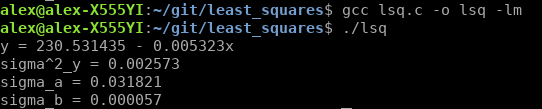
\includegraphics[width=0.7\linewidth]{runlsq}
\end{center}
\end{document}